\noindent

\includegraphics[height=1.25cm]{images/pictograms/benchmark}

\includegraphics[height=1.25cm]{images/pictograms/FDM}

\includegraphics[height=1.25cm]{images/pictograms/wave}

%%%%%%%%%%%%%%%%%%%%%%%%%%%%%%%%%%%%%%%%%%%%%%%%%%%%%%%%%%%%%%%%%%%%%%%%%%%%%%%%%%%%%%%%%%%%%%%%%%%

\begin{flushright} {\tiny {\color{gray} python\_codes/fieldstone\_166/text.tex}} \end{flushright}

%\lstinputlisting[language=bash,basicstyle=\small]{python_codes/template_keywords.key}

\par\noindent\rule{\textwidth}{0.4pt}

\begin{center}
\inpython
{\small Code: \url{https://github.com/cedrict/fieldstone/tree/master/python_codes/fieldstone_166}}
\end{center}

\par\noindent\rule{\textwidth}{0.4pt}

%%%%%%%%%%%%%%%%%%%%%%%%%%%%%%%%%%%%%%%%%%%%%%%%%%%%%%%%%%%%%%%%%%%%%%%%%%%%%%%%%%%%%%%%%%%%%%%%%%%

The theory and discretisation are described in Section~\ref{ss:fdmwavess}.


%------------------------------
\subsection*{Experiment \# 1}

The domain is $[0,1]$, $C_{CFL}=0.5$, $nnx=101$ and $c=1$.

\[
u(x,t) = \sin(\pi x) \cos(\pi c t)
\]

The initial wave field $u$ is as follows at $t=0$:
\begin{center}
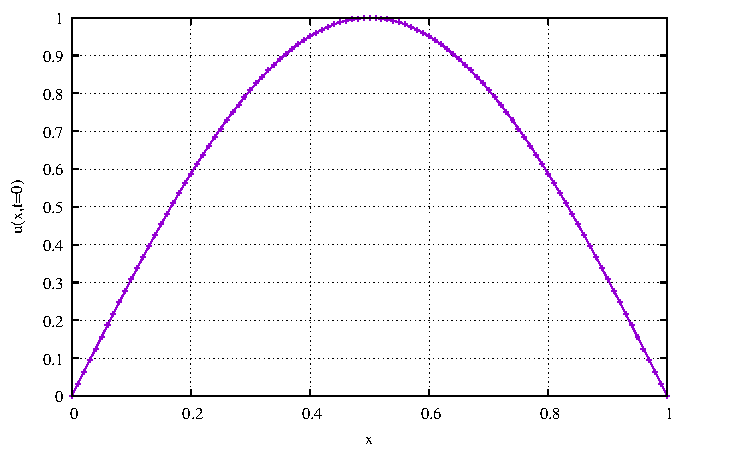
\includegraphics[width=7cm]{python_codes/fieldstone_166/RESULTS/exp1/u0.pdf}
\end{center}

The min/max values of $u$ as a function are as follows:
\begin{center}
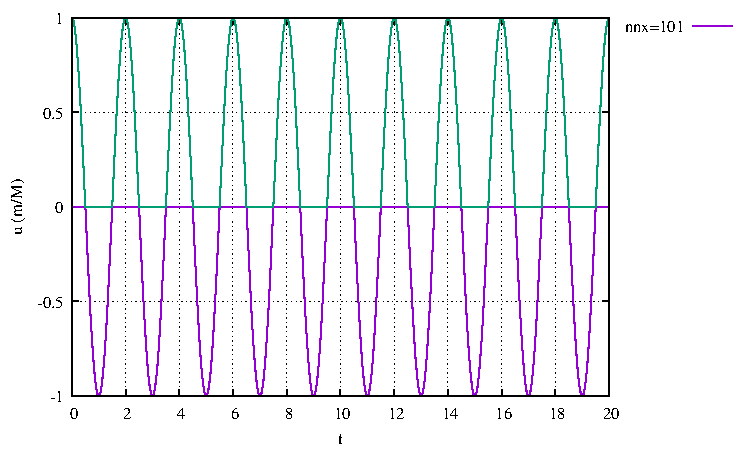
\includegraphics[width=7cm]{python_codes/fieldstone_166/RESULTS/exp1/u_stats.pdf}
\end{center}

The $u$ field is shown hereunder at three different times $t=5,10,15,20$:
\begin{center}
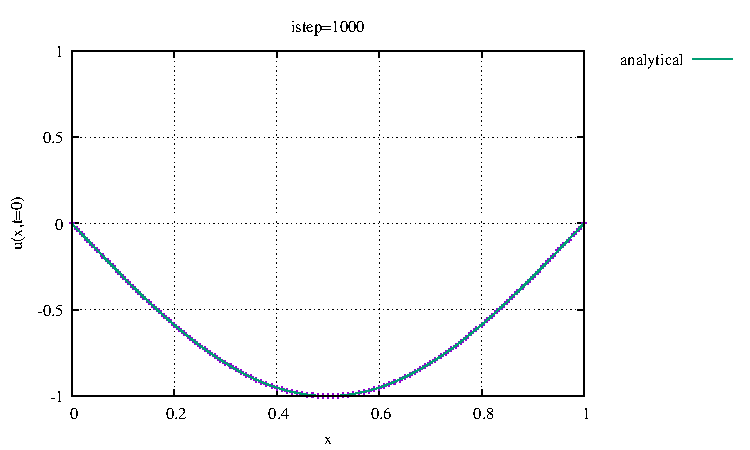
\includegraphics[width=7cm]{python_codes/fieldstone_166/RESULTS/exp1/u_1000.pdf}
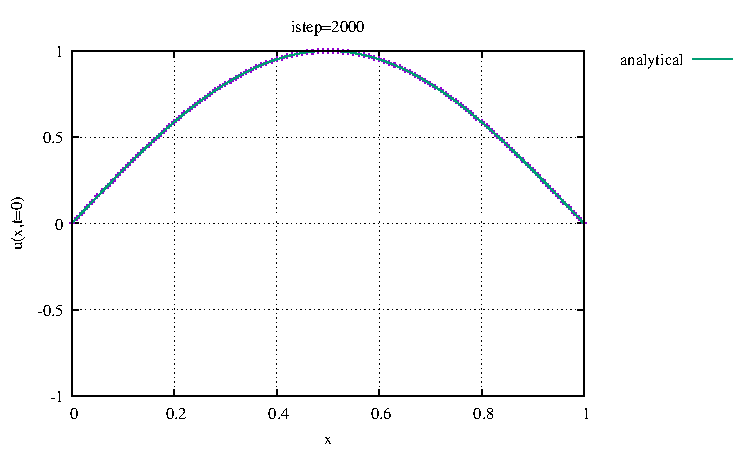
\includegraphics[width=7cm]{python_codes/fieldstone_166/RESULTS/exp1/u_2000.pdf}\\
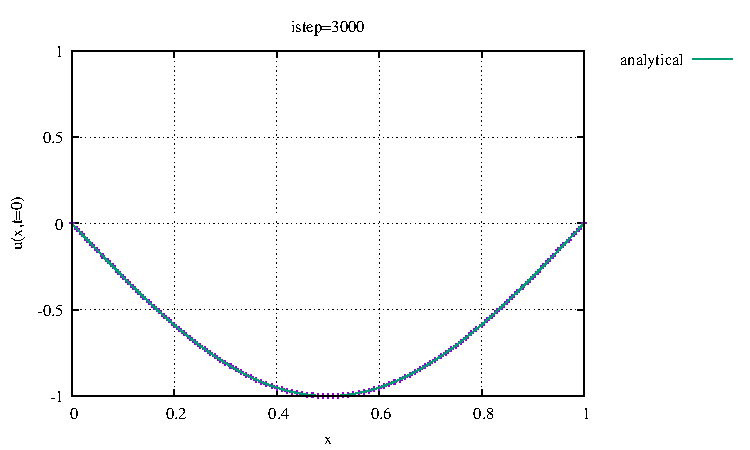
\includegraphics[width=7cm]{python_codes/fieldstone_166/RESULTS/exp1/u_3000.pdf}
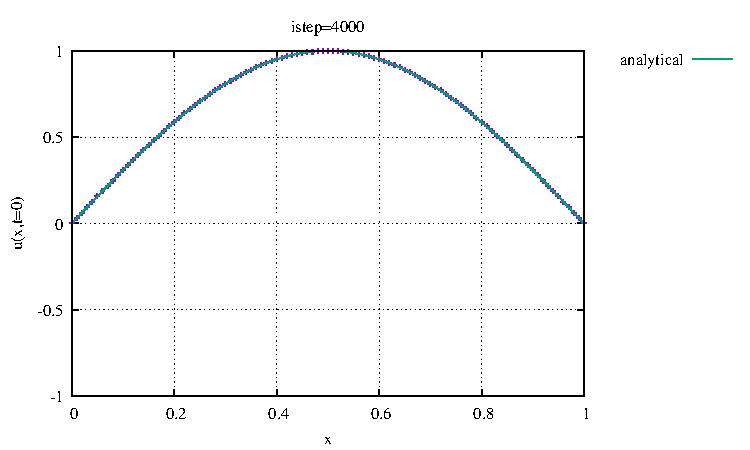
\includegraphics[width=7cm]{python_codes/fieldstone_166/RESULTS/exp1/u_4000.pdf}
\end{center}



